\documentclass{standalone}

\usepackage{tikz}
\usetikzlibrary{arrows}
\usetikzlibrary{decorations.markings}

\begin{document}

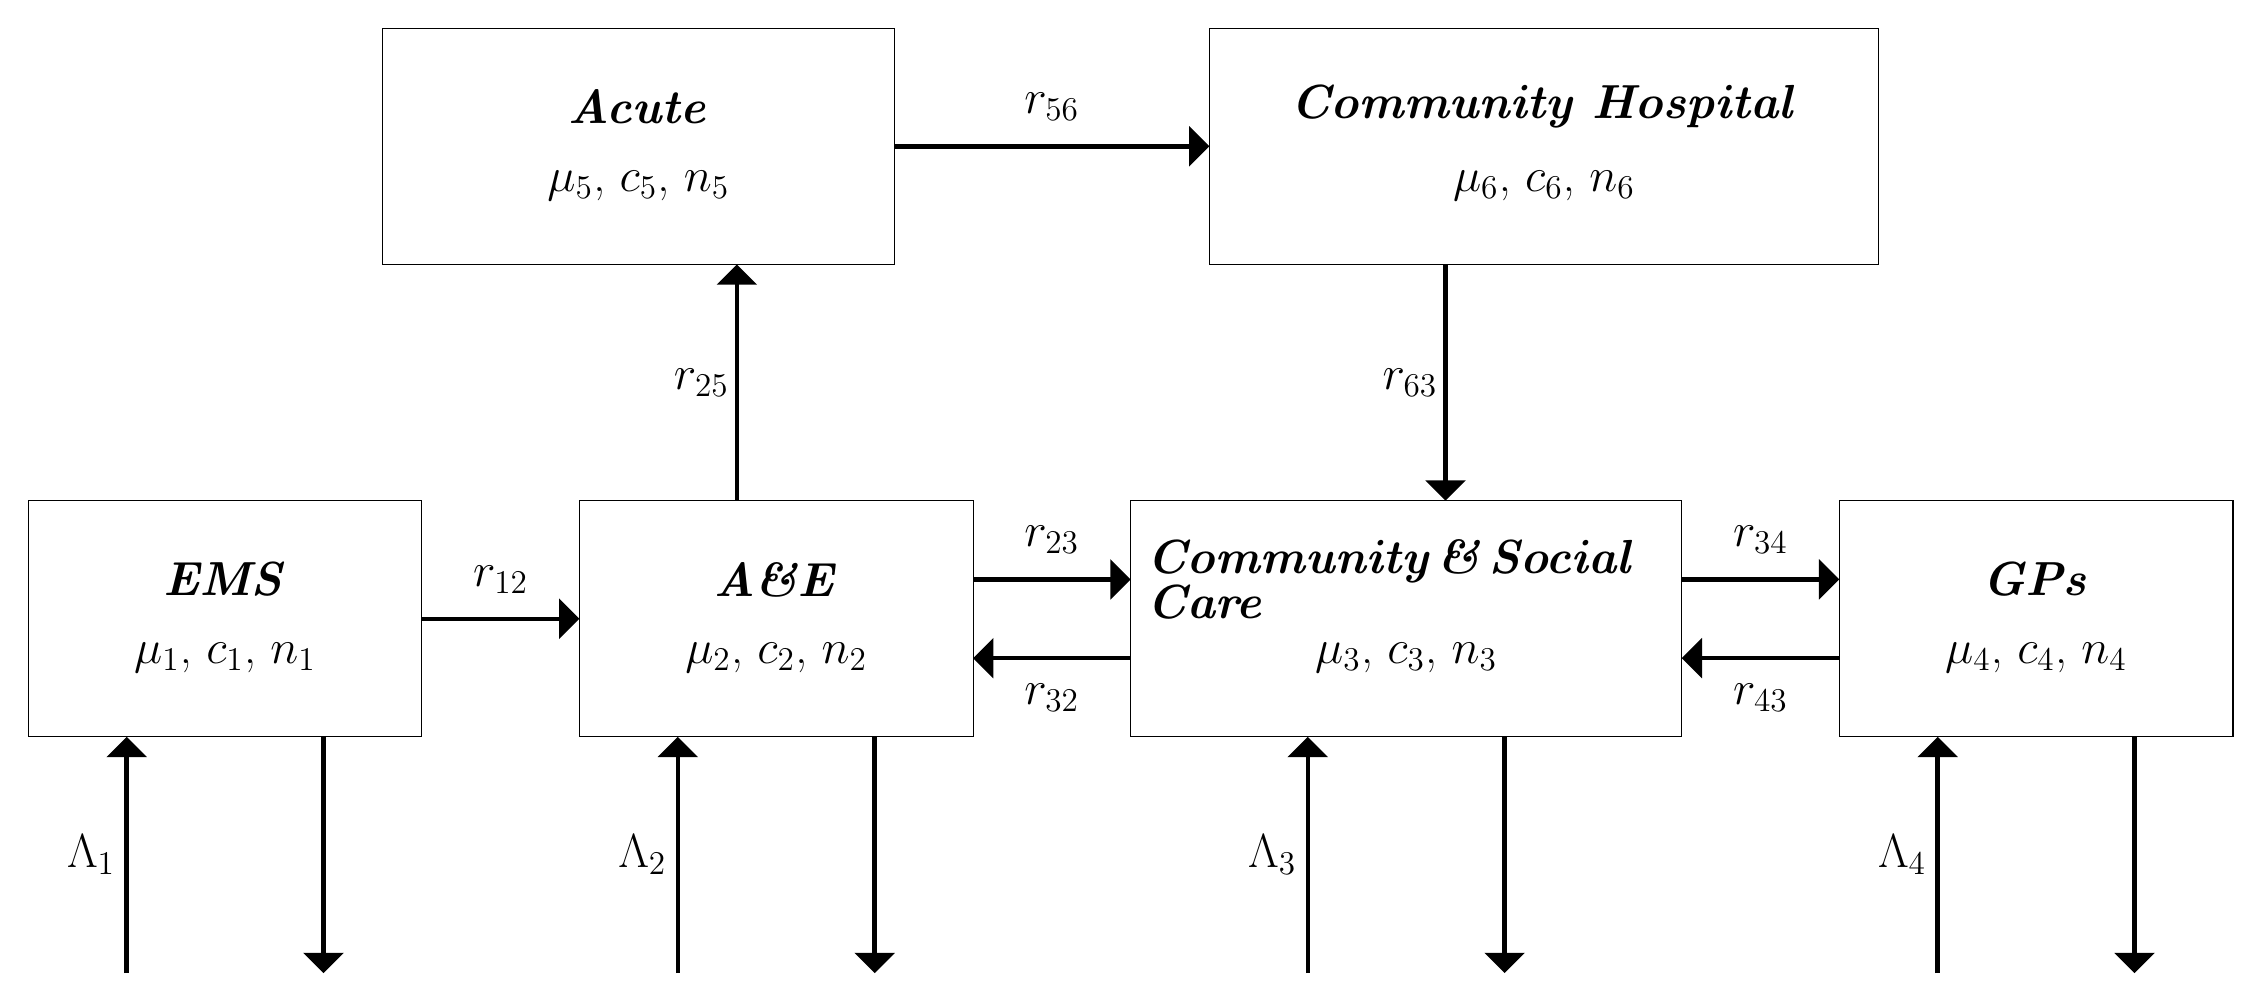
\begin{tikzpicture}

\draw (0, 3) -- (5, 3) -- (5, 0) -- (0, 0) -- cycle; % EMS
\node at (2.5, 2) {\LARGE{\textbf{\textit{EMS}}}};
\draw (7, 3) -- (12, 3) -- (12, 0) -- (7, 0) -- cycle; % A&E
\node at (9.5, 2) {\LARGE{\textbf{\textit{A\&E}}}};
\draw (14, 3) -- (21, 3) -- (21, 0) -- (14, 0) -- cycle; % Community / Social Care
\node[text width=200] at (17.72, 2) {\LARGE{\textbf{\textit{Community \& Social Care}}}};
\draw (23, 3) -- (28, 3) -- (28, 0) -- (23, 0) -- cycle; % GPs
\node at (25.5, 2) {\LARGE{\textbf{\textit{GPs}}}};
\draw (4.5, 6) -- (11, 6) -- (11, 9) -- (4.5, 9) -- cycle; % Acute
\node at (7.75, 8) {\LARGE{\textbf{\textit{Acute}}}};
\draw (15, 6) -- (23.5, 6) --(23.5, 9) -- (15, 9) -- cycle; % Community Hospital
\node at (19.25, 8) {\LARGE{\textbf{\textit{Community Hospital}}}};

\draw[ultra thick, -triangle 90] (5, 1.5) -- (7, 1.5); % EMS -> A&E
\draw[ultra thick, -triangle 90] (21, 2) -- (23, 2); % GPs -> Com/Soc
\draw[ultra thick, -triangle 90] (23, 1) -- (21, 1); % GPs <- Com/Soc
\draw[ultra thick, -triangle 90] (12, 2) -- (14, 2); % A&E -> Com/Soc
\draw[ultra thick, -triangle 90] (14, 1) -- (12, 1); % A&E <- Com/Soc
\draw[ultra thick, -triangle 90] (9, 3) -- (9, 6); % A&E -> Acute
\draw[ultra thick, -triangle 90] (11, 7.5) -- (15, 7.5); % Acute -> ComHosp
\draw[ultra thick, -triangle 90] (18, 6) -- (18, 3); % ComHosp -> Com/Soc

\draw[ultra thick, -triangle 90] (1.25, -3) -- (1.25, 0); % -> EMS
\draw[ultra thick, -triangle 90] (3.75, 0) -- (3.75, -3); % EMS ->
\draw[ultra thick, -triangle 90] (8.25, -3) -- (8.25, 0); % -> A&E
\draw[ultra thick, -triangle 90] (10.75, 0) -- (10.75, -3); % A&E ->
\draw[ultra thick, -triangle 90] (16.25, -3) -- (16.25, 0); % -> ComSoc
\draw[ultra thick, -triangle 90] (18.75, 0) -- (18.75, -3); % ComSoc ->
\draw[ultra thick, -triangle 90] (24.25, -3) -- (24.25, 0); % -> GPs
\draw[ultra thick, -triangle 90] (26.75, 0) -- (26.75, -3); % GPs ->

\node at (0.8, -1.5) {\LARGE{$\Lambda_{1}$}};
\node at (7.8, -1.5) {\LARGE{$\Lambda_{2}$}};
\node at (15.8, -1.5) {\LARGE{$\Lambda_{3}$}};
\node at (23.8, -1.5) {\LARGE{$\Lambda_{4}$}};


\node at (6, 2) {\LARGE{$r_{12}$}};
\node at (13, 2.5) {\LARGE{$r_{23}$}};
\node at (22, 0.5) {\LARGE{$r_{43}$}};
\node at (8.55, 4.5) {\LARGE{$r_{25}$}};


\node at (13, 0.5) {\LARGE{$r_{32}$}};
\node at (22, 2.5) {\LARGE{$r_{34}$}};
\node at (13, 8) {\LARGE{$r_{56}$}};
\node at (17.55, 4.5) {\LARGE{$r_{63}$}};
\node at (2.5, 1) {\LARGE{$\mu_1$, $c_1$, $n_1$}};
\node at (9.5, 1) {\LARGE{$\mu_2$, $c_2$, $n_2$}};
\node at (17.5, 1) {\LARGE{$\mu_3$, $c_3$, $n_3$}};
\node at (25.5, 1) {\LARGE{$\mu_4$, $c_4$, $n_4$}};
\node at (7.75, 7) {\LARGE{$\mu_5$, $c_5$, $n_5$}};
\node at (19.25, 7) {\LARGE{$\mu_6$, $c_6$, $n_6$}};



\end{tikzpicture}

\end{document}
